\section{差の理由を確かめる：相関と因果}

  \subsection{製作費をかければ多く見られるのか}

    前に, 製作費と視聴回数の散布図を, 縦横比だけ変えて二枚並べた.
    軸を引き伸ばすだけで, 傾きの印象が変わってしまう図だった.
    今度は縦横比に手を加えずに, 同じ点を一枚に打つ (\cref{fig:ch06-scatter}).

    \begin{figure}[htbp]
      \centering
      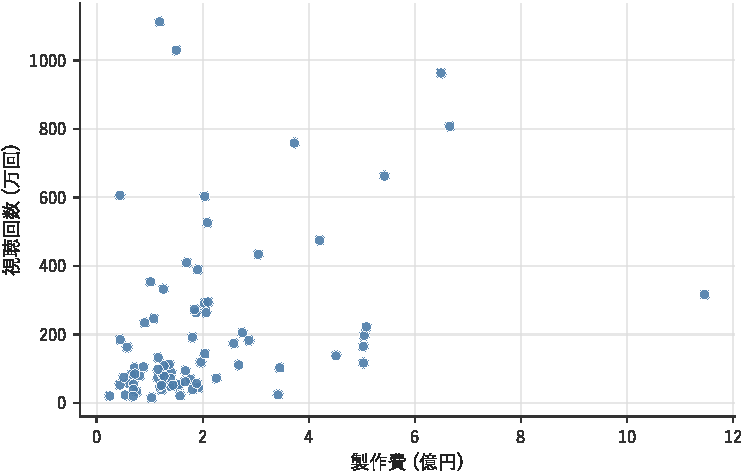
\includegraphics[width=0.7\linewidth]{../figures/output/ch03_scatter.pdf}
      \caption{製作費 (億円) を横軸に, 視聴回数 (万回) を縦軸に取り, 映画一本を一つの点で打った散布図. 縦横比は変えていない.}
      \label{fig:ch06-scatter}
    \end{figure}

    点は一直線には並んでいないが, 全体としては右上がりに見える.
    製作費の大きい映画では, 視聴回数も大きい傾向がある.
    このように, 一方が大きいものでは他方も大きい傾向があり, 散布図の点が右上がりに並ぶとき, 二つの数量には\textbf{相関}があるという.
    一方が大きいものでは他方が小さく, 点が右下がりに並ぶときも, 向きが逆の相関と呼ぶ.

    では, 製作費をかければ, そのぶん多く見られるのだろうか.
    この図からわかるのは, 製作費の大きい映画に視聴回数の大きいものが多い, ということまでだ.
    製作費の大きい映画は, 原作があるかどうかや宣伝の大きさも, 製作費の小さい映画と違っているかもしれない.
    そうだとすれば, 右上がりの一部は, 製作費ではなくそちらの違いから来ているかもしれない.

    原作の有無で映画を分けたときも, 事情は同じだった.
    原作のある映画のほうが平均視聴回数がおよそ120万回多く, 偶然とは説明しにくい差だと言えた.
    それでも, 原作があるから多く見られたとは言えなかった.
    相関があっても, 差があっても, それだけでは原因とは言えない.

    原作が原因だと言うには, 原作の有無だけが違っていて, ほかの条件がすべて揃っている二つの集まりを比べる必要があった.
    しかし, どうすればそんな集まりが手に入るだろうか.

    そもそも, ある一本の映画について「原作の効果」を確かめようとすると, 途端に行き詰まってしまう.
    その作品に本当に原作の効果があったのかを知るには, その映画を原作つきで公開したときの視聴回数と, まったく同じ映画を原作なしのオリジナル脚本で公開したときの視聴回数を比べる必要がある.
    二つの数字を引き算して差が残れば, それこそが原作の純粋な効果だと言えるはずだ.

    だが, 一本の映画を二度公開することはできない.
    見ることができるのは原作つきで世に出たほうの視聴回数だけで, 原作がなかった場合の視聴回数はどこにもないから, 一本ずつの作品について効果を直接測ることは誰にもできない.

    一本で比べられないのだとすれば, 集まりで比べるほかない.
    観測できるのは, 原作のある作品たちの平均視聴回数と, 原作のない作品たちの平均視聴回数だ.
    もしもこの二つの集まりが「原作の有無以外は同じ」であるなら, 二つの平均の差を, 原作がもたらした平均的な効果と考えて差し支えない.

  \subsection{くじで決める意味}

    前に信頼区間のところで触れた薬の治験に戻る.
    新しい薬を飲んだ集まりと, 飲んでいない集まりで血圧を比べたところ, 薬を飲んだほうが平均で 5\,mmHg 低く, 95\%信頼区間は 2\,mmHg から 8\,mmHg だった.
    このとき, 5\,mmHg という差を素直に「薬の効果」とみなしていた.
    映画では原作の効果だと言い切るのをためらったのに, なぜ治験の差なら効果だと受け取れたのだろうか.

    適切な治験では, 誰が薬を飲んで誰が飲まないかを, 医師や患者の希望ではなく, くじ引きで決める.
    このように, 集まりへの割り振りをくじなどの偶然に任せて分ける手続きを\textbf{無作為化}と呼ぶ.

    くじで分ければ, 年齢や性別, もともとの血圧の高さ, 日頃の生活習慣といったあらゆる要素が, 薬を飲むかどうかとはまったく無関係に二つの集まりへ散らばっていく.
    人数が十分に多ければ, 二つの集まりは, 薬を飲むかどうかという一点を除いて, ほかのあらゆる点でよく似た集まりになる.

    二つの集まりが薬以外の点ですでに似通っているのだから, あとから生じた血圧の差は, 薬を飲んだことによって生じた差だと考えるのが自然だ.
    だからこそ, 治験のデータから計算した標準誤差も, 信頼区間も, 検定の結果も, そのまま「薬の効果がどれくらいか」「効果が偶然のばらつきによるものではないか」の根拠として信頼することができた.

    この信用は, 差が 5\,mmHg だったという計算結果そのものから生まれたのではない.
    薬を飲む人と飲まない人をくじで分けた, という手順そのものが信用を支えている.

  \subsection{くじで分けられないデータ}

    ところが, 映画のデータに目を戻すと, 状況はまるで違っている.
    映画はくじ引きで原作つきになるかどうかが決まったわけではない.
    前章で見たように, 原作のある映画には多額の製作費や大規模な宣伝がつきやすく, 二つの集まりは最初から原作の有無以外の点でも違っている.
    平均の差の中には, 原作そのものの効果と, ほかの条件の違いがごちゃ混ぜになって入り込んでいるのだ.

    くじ引きで分けられていないデータを見るかぎり, 「原作の有無以外は同じような集まりだ」と信じるに足る根拠はどこにもない.
    それでもその差を原因によるものだと言いたいなら, 「ほかの条件に大きな違いはないはずだ」と自分で仮定を置いて比べるしかない.
    もしその仮定が外れていれば, 計算された差は原因とはまったく違うものを指し示してしまう.

    これまで見てきたように, 標本サイズを増やせば標準誤差は小さくなり, 信頼区間は狭くなって, 検定でも小さな差を有意と言えるようになる.
    だが, 標本をどれほど増やしてばらつきを小さくしても, 目に見える差と本当の効果とのあいだにある隔たりは少しも埋まらない.

  \subsection{条件をそろえて比べる}

    くじで分けることができないなら, できる手立ては何だろうか.
    一番素朴な方法は, 違っていそうな条件をそろえて比べることだ.

    たとえば, 製作費の違いが邪魔をしていると思うなら, 製作費が同じくらいの映画どうしを集めて, その中で原作のある作品とない作品の視聴回数を比べればよい.
    製作費の少ない作品の中だけで比べ, 次に製作費の多い作品の中だけで比べる, というように条件をそろえていけば, 少なくとも製作費の違いが差に混ざり込むことは防げる.
    このように, データを条件ごとにいくつかの層に分けて調べる手続きを層別と呼ぶ.

    ここで問題になっていた製作費のように, 原作の有無より先に決まっていて, 原作の有無にも視聴回数にも影響し, 見かけの差を狂わせてしまう第三の要因を\textbf{交絡}（あるいは\textbf{交絡因子}）と呼ぶ.
    条件をそろえて比べるというのは, この交絡を取り除くための作業だ.

    条件をそろえることで見え方が一変する様子は, 実際のデータでも確かめられている.
    1973年, カリフォルニア大学バークレー校の大学院で, 性別による入試の差別があるのではないかとして問題になったことがあった\footnote{Bickel, P. J., Hammel, E. A., \& O'Connell, J. W. (1975). Sex Bias in Graduate Admissions: Data from Berkeley. \textit{Science}, 187(4175), 398--404.}.
    全志願者の合格率を集計してみると, 男子の合格率は約44\%だったのに対し, 女子の合格率は約35\%で, 男子のほうが9ポイントほど高かった.
    全体だけを見れば, 男子のほうが受かりやすいように思える.

    ところが, 志願者を学部ごとに分けて合格率を計算し直してみると, まるで違う姿が現れた.
    主要な6つの学部のうち4つでは, 女子の合格率は男子と同じか, むしろ高かったのだ.
    残り2つの学部でも, 全体で出ていた9ポイントもの差は見られなかった.

    全体で9ポイントあった差は, どこへ消えてしまったのだろうか.
    実は, 学部ごとの合格率は一様ではなく, 合格率が6\%しかない狭き門の学部もあれば, 64\%もある受かりやすい学部もあった.
    そして女子の志願者は, 合格率の低い狭き門の学部に多く集まっており, 男子は合格率の高い学部に多く集まっていたのだ (\cref{fig:ch06-berkeley}).
    そのため, 学部をそろえずに全体をまとめて集計すると, 審査で男子のほうが有利に扱われているかのような差が出ていた.
    このように, 全体で見たときと分けて見たときとで差の向きが逆になったり差が消えたりする現象を, シンプソンのパラドックスと呼ぶ.

    \begin{figure}[htbp]
      \centering
      % 第6章 図6-1: バークレーの主要6学部の男女別の合格率 (上) と志願者数 (下)
% 学部別の数値は Bickel ほか (1975) の主要6学部 (R の UCBAdmissions と照合, 2026-09-27)
%   A: 男 825人 62.1%, 女 108人 82.4%   B: 男 560人 63.0%, 女  25人 68.0%
%   C: 男 325人 36.9%, 女 593人 34.1%   D: 男 417人 33.1%, 女 375人 34.9%
%   E: 男 191人 27.7%, 女 393人 23.9%   F: 男 373人  5.9%, 女 341人  7.0%
% 「全志願者」は本文の数値 (全学部: 男 約44%, 女 約35%)
\begin{tikzpicture}[font=\footnotesize]
  \begin{axis}[
    name=rate,
    width=0.82\linewidth, height=4.6cm, scale only axis=false,
    ybar, bar width=7pt,
    ymin=0, ymax=100, ytick={0,20,40,60,80,100},
    ylabel={合格率 (\%)},
    xmin=-0.7, xmax=6.7,
    xtick={0,1,2,3,4,5,6},
    xticklabels={全志願者,学部A,学部B,学部C,学部D,学部E,学部F},
    x tick label style={font=\footnotesize},
    axis x line*=bottom, axis y line*=left,
    legend style={draw=none, at={(0.98,0.98)}, anchor=north east, font=\footnotesize},
    legend image code/.code={\draw[#1] (0cm,-0.1cm) rectangle (0.3cm,0.1cm);},
    enlarge x limits=false,
  ]
    \addplot[draw=black, fill=black!15] coordinates {
      (0,44) (1,62.1) (2,63.0) (3,36.9) (4,33.1) (5,27.7) (6,5.9)};
    \addplot[draw=black, fill=black!65] coordinates {
      (0,35) (1,82.4) (2,68.0) (3,34.1) (4,34.9) (5,23.9) (6,7.0)};
    \legend{男子, 女子}
    \draw[black!40] (axis cs:0.5,0) -- (axis cs:0.5,100);
  \end{axis}
  \begin{axis}[
    at={(rate.south)}, anchor=north, yshift=-1.1cm,
    width=0.82\linewidth, height=3.2cm, scale only axis=false,
    ybar, bar width=7pt,
    ymin=0, ymax=900, ytick={0,300,600,900},
    ylabel={志願者数 (人)},
    xmin=-0.7, xmax=6.7,
    xtick={1,2,3,4,5,6},
    xticklabels={学部A,学部B,学部C,学部D,学部E,学部F},
    x tick label style={font=\footnotesize},
    axis x line*=bottom, axis y line*=left,
    enlarge x limits=false,
  ]
    \addplot[draw=black, fill=black!15] coordinates {
      (1,825) (2,560) (3,325) (4,417) (5,191) (6,373)};
    \addplot[draw=black, fill=black!65] coordinates {
      (1,108) (2,25) (3,593) (4,375) (5,393) (6,341)};
  \end{axis}
\end{tikzpicture}

      \caption{1973年のカリフォルニア大学バークレー校大学院の入試について, 主要6学部の合格率 (上) と志願者数 (下) を男女別に表した図. 左端の「全志願者」は主要6学部以外も含む全学部を合わせた合格率で, 右の6学部を合計したものではない. 学部別の数値は Bickel ほか (1975) による.}
      \label{fig:ch06-berkeley}
    \end{figure}

  \subsection{そろえてはいけない条件}

    条件をそろえれば交絡が防げるのだとしたら, 思いつく限りの条件をすべてそろえて比べればよいのだろうか.
    そろえるべきではない条件をそろえてしまうと, 今度は本物の効果を消し去ってしまうことがある.

    日常の健康を例に考えてみよう.
    運動の習慣がある人とない人で血圧を比べるとする.
    運動をすると体重が減り, その減った体重のおかげで血圧が下がっている, という関係があったとしよう.

    ここで, 「体重が違うと公平に比べられない」と考えて, 体重が同じくらいの人どうしを集めて運動の効果を比べたらどうなるだろうか.
    体重が同じ人たちの集まりの中では, 運動による「体重が減る」という効果が最初から封じ込められてしまっている.
    その結果, 運動している人と運動していない人のあいだに血圧の差は見られなくなってしまう.

    運動が効いていないわけではない.
    運動の効果は体重という通り道を通って現れていたのに, その体重をそろえてしまったために見えなくなったのだ.
    ここでの体重は, 交絡ではなく, 原因から結果へ至る道筋の途中にある.

    やっかいなのは, データの数字を見ているだけでは, ある条件が交絡なのか, それとも効果の通り道なのかを区別することはできない, という点だ.
    手元の表に並んでいる数字は, どちらの場合であってもまったく同じように見える.
    それを区別できるのは, 運動や体重や血圧が体の中でどう作用し合っているのかという, 現実の仕組みについての知識だけだ.

  \subsection{信用の根拠をどこに置くか}

    映画の分析に立ち返ってみよう.
    製作費はそろえるべきだろうか.
    原作があるから大きな製作費がつき, 宣伝も大きくなり, その結果として多く見られたのだとしたら, 製作費は交絡ではなく, 原作から視聴回数への通り道にある.
    製作費をそろえて比べることは, 体重をそろえて運動の効果を消したのと同じことになってしまう.

    どちらなのかは, 手元の数字からは決まらない (\cref{fig:ch06-paths}).
    企画が立ち上がり, 予算がつき, 宣伝され, 観客に届くまでの仕組みについての知識から考えるほかない.

    \begin{figure}[htbp]
      \centering
      % 第6章 図6-2: 製作費が交絡になる場合 (左) と通り道になる場合 (右)
% 箱と数字は同じで, 違うのは矢印の向きだけ
\begin{tikzpicture}[
    font=\small,
    box/.style={draw, rounded corners=2pt, minimum width=2.1cm, minimum height=0.75cm, fill=black!5},
    arr/.style={-stealth, thick, shorten >=1pt},
  ]
  % 左: 製作費が原作の有無と視聴回数の両方に先立つ
  \node[box] (L-cost) at (0,1.6) {製作費};
  \node[box] (L-src)  at (-1.9,0) {原作の有無};
  \node[box] (L-view) at (1.9,0) {視聴回数};
  \draw[arr] (L-cost) -- (L-src);
  \draw[arr] (L-cost) -- (L-view);
  \draw[arr] (L-src) -- (L-view);
  \node[font=\footnotesize] at (0,-0.9) {交絡になる場合};
  % 右: 原作から製作費を通って視聴回数へ
  \begin{scope}[xshift=7.2cm]
    \node[box] (R-cost) at (0,1.6) {製作費};
    \node[box] (R-src)  at (-1.9,0) {原作の有無};
    \node[box] (R-view) at (1.9,0) {視聴回数};
    \draw[arr] (R-src) -- (R-cost);
    \draw[arr] (R-cost) -- (R-view);
    \draw[arr] (R-src) -- (R-view);
    \node[font=\footnotesize] at (0,-0.9) {通り道になる場合};
  \end{scope}
\end{tikzpicture}

      \caption{製作費が交絡になる場合 (左) と, 原作の有無から視聴回数への通り道になる場合 (右) を, 矢印で表した図. 矢印は, 根元にあるものが矢印の指すものに影響することを表す. 左右で違うのは, 製作費と原作の有無を結ぶ矢印の向きだけである.}
      \label{fig:ch06-paths}
    \end{figure}

    仕組みから考えて製作費が交絡なら (左の図), 製作費をそろえて比べる必要がある.
    そろえずに比べた差には, 製作費の違いから来た分が混ざってしまうからだ.

    製作費が通り道なら (右の図), そろえると消えてしまうのは, 原作の効果のうち製作費を通って現れる分だ.
    その分まで含めた効果を知りたいなら, 製作費をそろえてはいけない.
    それを除いた効果を知りたいなら, そろえてかまわない.
    製作費をそろえずに比べたときの差は, 原作がついたことで製作費や宣伝まで大きくなった分も込みの効果だ.
    製作費をそろえて比べたときの差は, 製作費が同じだったとしたら原作の名前だけでどれだけ違うか, という効果になる.
    どちらも意味のある数だが, 同じ数ではない.
    何を知りたいのかを決めないと, そろえる条件も決まらない.

    バークレーの入試の学部も, 実は通り道のほうに近い.
    学部は性別より先に決まっていたわけではなく, 志願者が自分で選んで出願したものだ.
    性別によって志願する学部が違い, 学部によって合格率が違う, という並びは, 運動と体重と血圧の並びと同じ形をしている.
    それなら, 学部をそろえて比べたのはまずかったのだろうか.

    当時問題になっていたのは, 審査で女子が不利に扱われていないか, ということだった.
    審査は学部ごとに行われるので, 審査での扱いを確かめるなら, 同じ学部の志願者どうしで比べるのが筋だ.
    学部をそろえて比べたのは, 知りたいことに合っていたのだ.
    この件を調べた研究者たちも, 審査で女子が不利に扱われていたとは言えず, 全体の差は女子が狭き門の学部に多く出願していたことから生じた, と結論している.

    一方, 女子の志願が狭き門の学部に集まっていること自体を問題にするなら, 全体の9ポイントの差にも意味がある.
    女子であることが, 学部選びまで含めて合格の機会をどれだけ狭めているかを表す数になるからだ.
    ただし, その差を生んだのは審査ではなく, どの学部に志願するかの偏りと, その偏りの背景にある事情だ.

    それでもなお, くじ引きで分けた治験から得られた差と, ほかの条件をそろえて比べた映画の差とでは, 置いている信用の種類が根本から異なっている.
    治験の差は, くじ引きで分ければ二つの集まりが揃うからこそ, その手順の確かさを根拠にして信じることができた.
    一方, 映画のようにくじで分けられないデータから得られた差は, 「必要な条件はすべてそろえたはずだ」という仮定に支えられているにすぎない.
    原因を確かめるにはほかの条件がすべて揃っている集まりが要ると言ったが, 通り道になっている条件までそろえれば本物の効果まで消えてしまうことがあるので, 「すべて」は言いすぎだった.
    残りの条件をすべてそろえることも, 実際にはできない.
    できるのは, 差を狂わせそうな条件を思いつくかぎり挙げ, そのうち測れたものをそろえることだけだ.
    もし見落とした条件が一つでも残っていれば, 導き出された結論はいつでも揺らぎうるのだ.

  \begin{mybox}{ここまででわかったこと}
    四段階の四つ目「仮定を確かめて判断する」.

    \textbf{この章で言えるようになったこと}: 製作費と視聴回数に相関があっても, 製作費をかけたから多く見られたとは言えない.
    治験の $5\,\mathrm{mmHg}$ の差を薬の効果と考えられたのは, 飲む人と飲まない人をくじで分けたからだった.
    くじで分けていない映画の約120万回の差を原作の効果と言うには, ほかの必要な条件がそろっているという仮定が要る.

    \textbf{まだ言えないこと}: 比べる作品の条件をそろえても, そもそも手元の80本が人気作ばかりだったらどうだろうか.
    この80本から作品全体のことが言えるかは, まだ確かめていない.

    \textbf{前の章の見方がどう変わったか}: 本数を増やせば差の区間は狭くなるが, それだけでは原作の効果に近づかない.
  \end{mybox}
